\documentclass[sn-mathphys,Numbered]{sn-jnl}
\usepackage{graphicx}%
\usepackage{multirow}%
\usepackage{amsmath,amssymb,amsfonts}%
\usepackage{amsthm}%
\usepackage{mathrsfs}%
\usepackage[title]{appendix}%
\usepackage{xcolor}%
\usepackage{textcomp}%
\usepackage{manyfoot}%
\usepackage{booktabs}%
\usepackage{algorithm}%
\usepackage{algorithmicx}%
\usepackage{algpseudocode}%
\usepackage{listings}%
\usepackage{float}
\usepackage[font=small,labelfont=bf]{caption}
\setlength{\parskip}{0.25\baselineskip}


\newcommand{\supp}{{\text{supp}}} 
\newcommand{\bv}{{\text{BV}}}
\newcommand{\ac}{{\text{AC}}}

\newenvironment{problem}[2][]{\begin{trivlist}
\item[\hskip \labelsep {\bfseries #1}\hskip \labelsep {\bfseries #2.}]}{\end{trivlist}}

\begin{document}

\title{An overview on $k$-medians clustering and procedurally determining $k$}

\author{Maxence Garcia, Alexandra M. Scott, Eric Tao}

\affil{ \orgname{Tufts University}}

\abstract{Clustering methods are important in unsupervised learning methods in order to determine patterns in large data sets. However, real-world data may include noise, may not be normally distributed, and the value of $k$ is not necessarily a priori obvious. We discuss using $k$-medians as an alternative to $k$-means clustering as one way to combat statistical noise as well as methods to procedurally compute reasonable values for $k$.}
\maketitle

\section{Introduction}

Clustering methods are unsupervised machine learning techniques that attempt to group together data points into partitions based off of minimizing some cost function. In class, we have seen methods such as hierarchical clustering via some choice of a distance function (single and complete linkage), $k$-means which tries to create $k$ clusters where the sum of distances between cluster centroids and points is minimal across all clusters, and DBSCAN, which attempts to geometrically categorize points.

In our case, we will be focusing on $k$-means and variations of that algorithm. We notice that a key feature of this algorithm is the reliance on means. However, in many real-world cases, data sets tend to have noise, potentially due to an artifact of data collection, the constraints on the data set distorting the distribution (i.e. being non-negative), or large outliers distorting the mean. 

In such cases, $k$-medians is a method that may be more robust to such statistical artifacts. Instead of determining the mean of each cluster, we may consider the two possibilities, the geometric median and the component-wise median. Both are reasonable choices in order to reduce the effects of large outliers, and, mathematically, this has the effect of minimizing the $L^1$ distances.

Further, we note that the value of $k$, the number of clusters, is not so obviously known a priori to clustering methods. In $k$-means, some methods that have been used to good effect include the elbow method, the Silhouette method, and the Gap statistic. For example, the elbow method runs $k$-means for various values of $k$, and computes the total distances between cluster points and the respective centroid. Since of course, as $k \to n$ for $n$ the count of our data points, this metric goes to $0$ as in that case, every point is its own centroid. Then, instead, the elbow method takes $k$ to be the smallest $k$ such that $k+1$ is a relatively small decrease in the total distance. 

\section{Framework}

\subsection{Context}

We first recall the overall setting in which we are working in. Let $\{ x_i \}_{i=1}^n \subset \mathbb{R}^D$ be a set of $D$-dimensional data points, or observations. We wish to assign to these data points $y_1,...,y_k$ labels corresponding to clusters $C_1,...,C_k$, for some fixed $1 \leq k < n$, such that some loss function is minimized across all potential assignments.

In the $k$-means context, our loss function was realized as the $L^2$ norm or Euclidean norm. If we defined a cluster as  $C_i = \{ x_j : y_j = i \}$, then our loss function here is simply:

$$ F(C_1,...,C_k) = \sum_{j=1}^k \left( \sum_{x_i \in C_j} \Vert x_i - \mu_j \Vert_2^2 \right) =  \sum_{j=1}^k \sum_{x_i \in C_j} \left\Vert x_i - \frac{1}{|C_j|}\sum_{x_l \in C_j} x_l \right\Vert_2^2 $$

where we use the distance between data points in the cluster to the mean $\mu_j$ of the cluster $C_j$.

Although there is strong geometric interpretation here, we notice that from a statistical standpoint, it is well known that the mean is not resistant to outliers. Indeed, consider an outlier point, that is, suppose there exists $x^o = x_j$ such that $\Vert x_i - x^o\Vert_2^2 > \delta$ for all $x_i \not = x_j$. In particular, since we have a finite set of points, it must be bounded. Let $M$ be the upper bound for the norms other than the outlier, $\{ \Vert x_i \Vert : i \not = j \}$, and choose $\delta > Mn$ for example. Then, we must have that this outlier is a point on its own, as including it in any cluster with other points will incur a penalty of at least $Mn$, and the other points may only be at most $M$ away from the origin. 

Although this is not necessarily detrimental to the algorithm, as some outliers such as these should be removed in a data cleaning step, in other cases of sampling data from distributions with long tails, this may result in incorrect clustering. Analogously to usual statistical methods then, we introduce the median as an alternative choice of centroid, more resistant to outliers, that can be used with such noisy distributions and sampling.

\subsection{Definitions}

Firstly, we will define the median that we will be using. Let $\{ x_i \}_{i=1}^n \subset \mathbb{R}^D$ be a set of points, and define the median as:

$$ m = \arg \min \sum_{i=1}^n | x_i - y | \implies m_j =  \arg \min \sum_{i=1}^n | (x_i)_j - y_j | $$

that is, the component-wise median of the points in the cluster. We may recognize this also as the $L^1$ norm.

In a similar fashion then, we may define our loss functional as being:

$$F(C_1,...,C_k) = \sum_{j=1}^k \left( \sum_{x_i \in C_j} \Vert x_i - m_j \Vert_2^2 \right)$$

where, as last time, $m_j$ corresponds to the median of the cluster $C_j$.

It may be useful to have an understanding of why this corresponds to a median, and how this relates to the intuitive definition of a median being the "middle value". Recall that geometrically, $|x - y|$ is symmetric around $x = y$, where the value of that function is $0$. Thus, the minimum value of $ \sum_{i=1}^n \sum_{j=1}^D | (x_i)_j - y_j | $ must be $y_j$ such that the $(x_i)_j$ values are "balanced" in a way around $y_j$; that is, we must have that $\sum_{(x_i)_j > y_j} |  (x_i)_j - y_j| = \sum_{(x_i)_j < y_j} |  (x_i)_j - y_j|$ for $y_j$ achieving the minimum.

From here, we proceed in the same way as the normal $k$-means algorithm. We choose arbitrary starting cluster centroids, with some heuristic for reasonableness. Then, we iteratively update the cluster points by adding data points to each cluster such that the overall functional is minimized.

\subsection{Choosing the value of $k$}

Here, we use the silhouette method as a heuristic for determining the value of $k$. At a high level, the silhouette method is an evaluation of how well points are clustered. Each point is assigned a score between $[-1,1]$, where a high score represents a high degree of similarity to the rest of the cluster as opposed to other clusters, and a low score is the opposite. The overall silhouette score can then determined as the average of the score across points. Formally, we define the silhouette score for a point $x_i$ as:

$$s(x_i) =  \frac{d(x_i, C_i) - d(x_i, C_j)}{\max\{ d(x_i, C_i) , d(x_i, C_j)\}}$$

where $d(x_i, C_k) = \sum_{x_k \in C_k} \Vert x_i  - x_k \Vert$, the summed distance between a point and every point in a cluster, $C_i$ is the cluster that $x_i$ belongs to, and $C_j$ is the cluster that is "closest" to $x_i$, that is, such that $d(x_i,C_k)$ is minimized for $k \not = i$.

In this sense, if there are points with low scores, there are outlier in the cluster, and there may be a better choice of $k$.

We notice that in this formulation, the choice of norm can be easily adjusted to fit the metric that we wish to use. Under $k$-medians, we can easily work with the $L^1$ norm instead of the $L^2$ norm that $k$-means works with, and we may use an analogous heuristic to guide our choice of optimal $k$.

\section{Synthetic data examples}

\subsection{Procedure}

In what follows is some analysis on a synthetic data set, generated with skewness. In particular, we sample 100 points in each category as follows:

$$ x_1: \begin{cases} \mu: (1,0) \\ \sigma = 0.5 \\ \tilde{\mu}_3 = -1 \\ g = 5 \end{cases} $$

$$ x_2: \begin{cases} \mu: (-1,0) \\ \sigma = 1 \\ \tilde{\mu}_3 = 2 \\ g = 10 \end{cases} $$

$$ x_3: \begin{cases} \mu: (0,-1) \\ \sigma = 1 \\ \tilde{\mu}_3 = 2 \\ g = 10 \end{cases} $$

where $\sigma$, the standard deviation is taken independently in the $x,y$ directions, $\tilde{mu}_3$, the skewness or third moment is taken independently as well, and same for $g$ the kurtosis.

\subsection{Data Visualization}

The definitions for the above are not important, but visualizing this, we can see that these points are very much not normally distributed:

\begin{center}
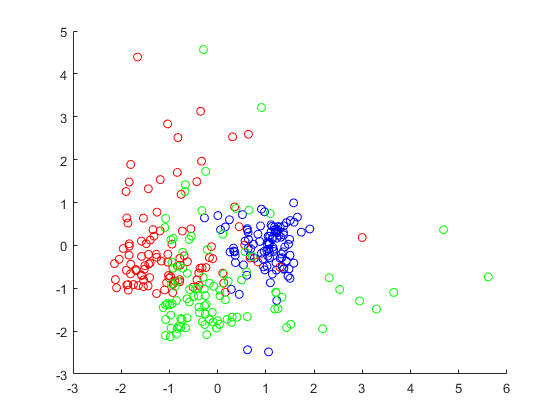
\includegraphics[width=\linewidth]{actual_clusters}
\captionof{figure}{Actual clusters}
\end{center}

Using $k$-means, we use a silhouette heuristic to try to determine a good value of $k$:

\begin{figure}[H]
\centering
\begin{minipage}{.5\textwidth}
  \centering
  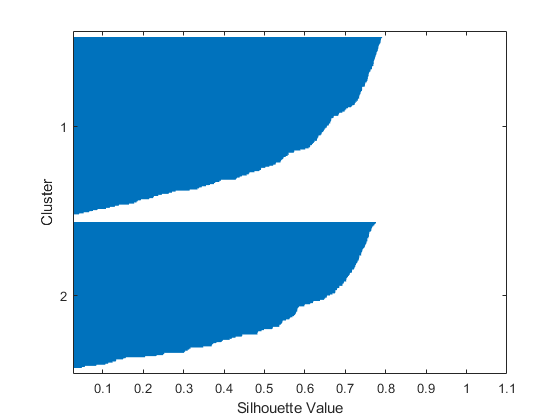
\includegraphics[width=\linewidth]{silhouette_means_2}
  \captionof{figure}{Silhouette under k-Means, $k=2$}
  \label{fig:test1}
\end{minipage}%
\begin{minipage}{.5\textwidth}
  \centering
  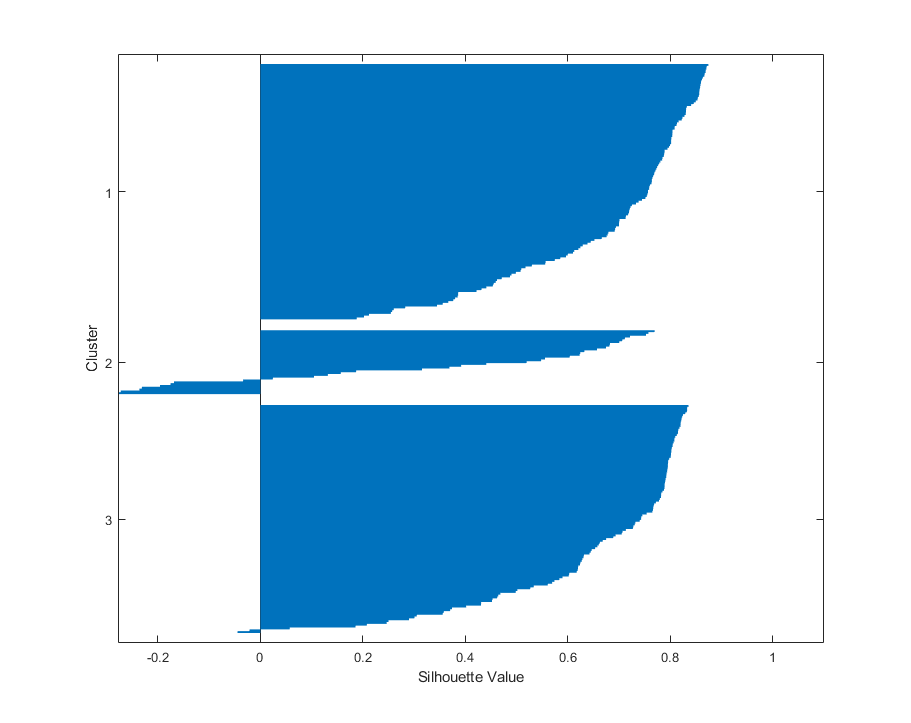
\includegraphics[width=\linewidth]{silhouette_means_3}
  \captionof{figure}{Silhouette under k-Means, $k=3$}
  \label{fig:test2}
\end{minipage}
\end{figure}

\begin{figure}[H]
\centering
\begin{minipage}{.5\textwidth}
  \centering
  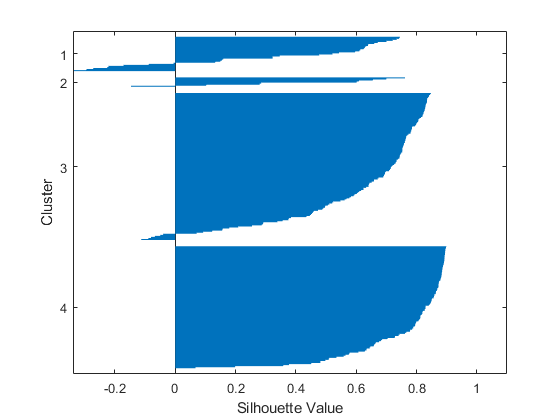
\includegraphics[width=\linewidth]{silhouette_means_4}
  \captionof{figure}{Silhouette under k-Means, $k=4$}
  \label{fig:test1}
\end{minipage}%
\begin{minipage}{.5\textwidth}
  \centering
  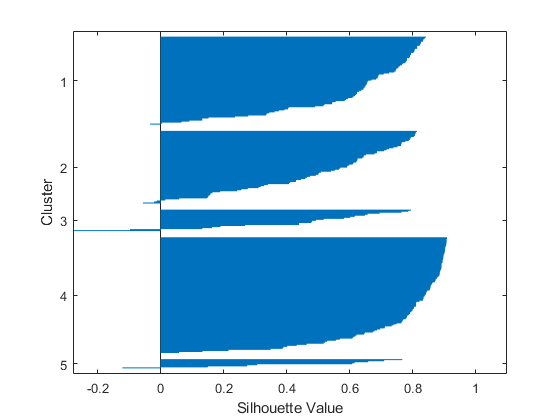
\includegraphics[width=\linewidth]{silhouette_means_5}
  \captionof{figure}{Silhouette under k-Means, $k=5$}
  \label{fig:test2}
\end{minipage}
\end{figure}

This comes with the following values of the sum of silhouettes:

\begin{center}
\begin{tabular}{|| c| c||}
\hline
k & Silhouette \\

\hline \hline
2 & 174.8 \\ \hline
3 & 194.8 \\ \hline
4 & 175.5 \\ \hline
5 & 190.9 \\ \hline
\end{tabular}
\end{center}

This implies that we should cluster with $k  = 3$ under $k$-means, and we recover the following clusters:

\begin{center}
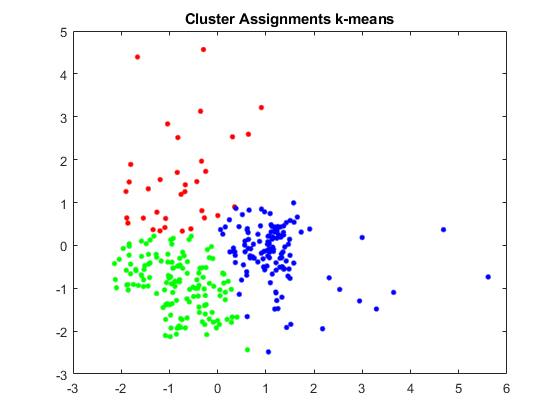
\includegraphics[width=\linewidth]{k_means_clusters}
\captionof{figure}{3-means clusters}
\end{center}

On the other hand, we repeat this for medians:

\begin{figure}[H]
\centering
\begin{minipage}{.5\textwidth}
  \centering
  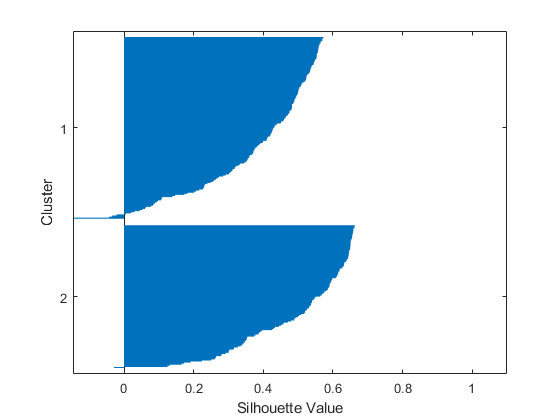
\includegraphics[width=\linewidth]{silhouette_medians_2}
  \captionof{figure}{Silhouette under k-Medians, $k=2$}
  \label{fig:test1}
\end{minipage}%
\begin{minipage}{.5\textwidth}
  \centering
  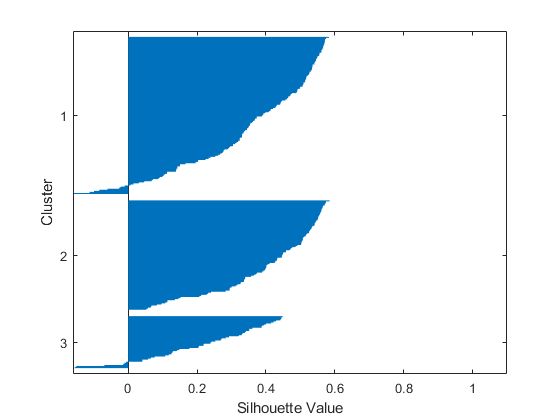
\includegraphics[width=\linewidth]{silhouette_medians_3}
  \captionof{figure}{Silhouette under k-Medians, $k=3$}
  \label{fig:test2}
\end{minipage}
\end{figure}

\begin{figure}[H]
\centering
\begin{minipage}{.5\textwidth}
  \centering
  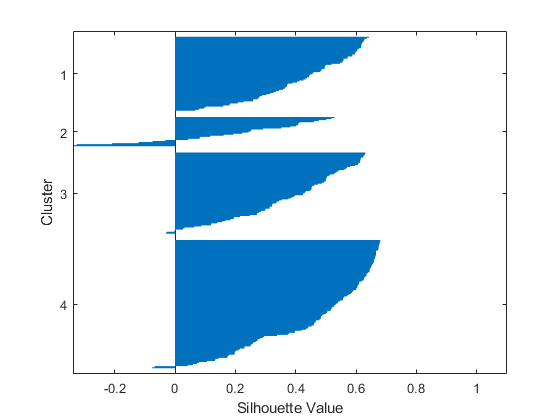
\includegraphics[width=\linewidth]{silhouette_medians_4}
  \captionof{figure}{Silhouette under k-Medians, $k=4$}
  \label{fig:test1}
\end{minipage}%
\begin{minipage}{.5\textwidth}
  \centering
  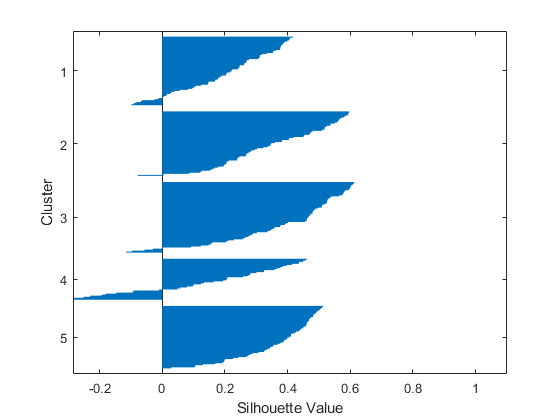
\includegraphics[width=\linewidth]{silhouette_medians_5}
  \captionof{figure}{Silhouette under k-Medians, $k=5$}
  \label{fig:test2}
\end{minipage}
\end{figure}

With, again, the sum of silhouette values:

\begin{center}
\begin{tabular}{|| c| c||}
\hline
k & Silhouette \\

\hline \hline
2 & 119.0 \\ \hline
3 & 126.5 \\ \hline
4 & 119.1 \\ \hline
5 & 91.3 \\ \hline
\end{tabular}
\end{center}

This implies we should run $k$-medians with $k=3$, and we find:

\begin{center}
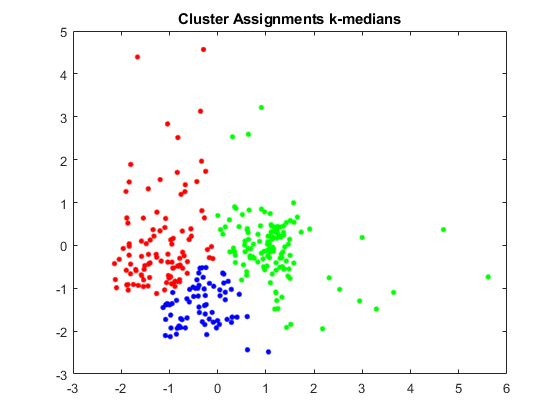
\includegraphics[width=\linewidth]{k_medians_clusters}
\captionof{figure}{3-medians clusters}
\end{center}

\section{Discussion}

We notice that qualitatively, the median and mean clustering differ heavily near $(-1,-1)$. Means tends to be pulled with the large outliers near $(-1,3)$, skewing the red cluster, while medians doesn't weight those points as much.

A remark, that rerunning the sum of silhouettes with k-medians tended to produce different results on each run. There may be some instability in terms of picking a suitable base point to start the $k$-medians algorithm from, and, as such, there can be variability in using the Silhouette heuristic on choosing the globally optimal value for $k$.

In general, we note that choosing $k$-medians can lead to better results in certain cases with large skewness or kurtosis, but does not necessarily coincide with $k$-means in general cluster location or even in the choice of $k$. Rather, it should be thought of as another tool that may be suitable for datasets where we have a strong indication via some heuristic or theory that the underlying data is not normal.

Further, we see from the Silhouette method, a powerful tool in classifying the efficacy of our clustering technique. In particular, we can see that for large $k$, that we found large negative values for some of the clusters. We can interpret this as meaning that even though the overall loss function is decreasing, that on the other hand, the characteristic of being associated uniquely to a single cluster starts to become very fuzzy, especially on certain boundaries. Of course, there are other methods to produce heuristics on choosing $k$, this being one of many.

\section{Bibliography}

Cardot, Hervé, Peggy Cénac, and Jean-Marie Monnez. "A fast and recursive algorithm for clustering large datasets with k-medians." Computational Statistics \& Data Analysis 56.6 (2012): 1434-1449.

Fischer, Aurélie. "On the number of groups in clustering." Statistics \& Probability Letters 81.12 (2011): 1771-1781.

Godichon-Baggioni, Antoine, and Sobihan Surendran. "A penalized criterion for selecting the number of clusters for K-medians." arXiv preprint arXiv:2209.03597 (2022).



\end{document}